\ifgerman{\chapter{Anhang}}{\chapter{Appendix}}
\label{appedixa}

\section{Difficulty Rating vs Time measurements co-relation}
\label{sanityCheck}
Sanity check is made to ensure that the assumption made from the results of difficulty rating hold true. To conduct the sanity check, we plot graphs with difficulty rating against time taken to answer a question, per interviewee.

\begin{figure}[H]
\centering
\begin{adjustbox}{width=1\textwidth}
\begin{minipage}[8cm]{.44\textwidth}
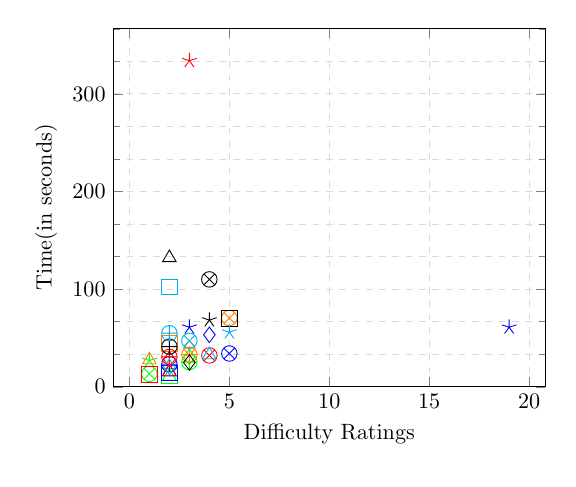
\begin{tikzpicture}[scale=0.80]
	\begin{axis}[%
	xlabel={Difficulty Ratings},
    ylabel={Time(in seconds)},
    ymin=0,
    minor y tick num=2,
    grid style={dashed,gray!30},
    ymajorgrids=true,
    xmajorgrids=true,
    yminorgrids=true,
    only marks,
    scatter,
    mark size=3.5pt,
    scatter src=explicit symbolic,
	scatter/classes={
		a={mark=square,draw=gray},
		b={mark=triangle,draw=gray},
		c={mark=otimes,draw=gray},
		x={mark=diamond,draw=gray},
	    y={mark=oplus,draw=gray},
		z={mark=star,draw=gray},
		q1sRa={mark=square,draw=green},
	    q1sT={mark=triangle,draw=green},
		q1sRo={mark=otimes,draw=green},
		q1cRa={mark=diamond,draw=green},
	    q1cT={mark=oplus,draw=green},
		q1cRo={mark=star,draw=green},
		q2sRa={mark=square,draw=orange},
	    q2sT={mark=triangle,draw=orange},
		q2sRo={mark=otimes,draw=orange},
		q2cRa={mark=diamond,draw=orange},
	    q2cT={mark=oplus,draw=orange},
		q2cRo={mark=star,draw=orange},
		q3sRa={mark=square,draw=blue},
	    q3sT={mark=triangle,draw=blue},
		q3sRo={mark=otimes,draw=blue},
		q3cRa={mark=diamond,draw=blue},
	    q3cT={mark=oplus,draw=blue},
		q3cRo={mark=star,draw=blue},
		q4sRa={mark=square,draw=red},
	    q4sT={mark=triangle,draw=red},
		q4sRo={mark=otimes,draw=red},
		q4cRa={mark=diamond,draw=red},
	    q4cT={mark=oplus,draw=red},
		q4cRo={mark=star,draw=red},
		q5sRa={mark=square,draw=black},
	    q5sT={mark=triangle,draw=black},
		q5sRo={mark=otimes,draw=black},
		q5cRa={mark=diamond,draw=black},
	    q5cT={mark=oplus,draw=black},
		q5cRo={mark=star,draw=black},
		q6sRa={mark=square,draw=cyan},
	    q6sT={mark=triangle,draw=cyan},
		q6sRo={mark=otimes,draw=cyan},
		q6cRa={mark=diamond,draw=cyan},
	    q6cT={mark=oplus,draw=cyan},
		q6cRo={mark=star,draw=cyan}},]
	\addplot[scatter,only marks,%
		scatter src=explicit symbolic]%
	table[meta=label] {
x         y         label
2	11.21	q1sRa
2	10.679	q1sT
1	13.292	q1sRo
		
3	30.59	q1cRa
3	25.252	q1cT
1	26.866	q1cRo
		
		
2	44.209	q2sRa
1	27.535	q2sT
5	70.4	q2sRo
		
3	39.415	q2cRa
3	32.897	q2cT
		
		
2	13.983	q3sRa
2	15.166	q3sT
5	34.07	q3sRo
		
4	53.26	q3cRa
2	23.036	q3cT
3	61.0	q3cRo
		
		
19

1	12.843	q4sRa
2	15.801	q4sT
4	32.092	q4sRo
		
2	28.282	q4cRa
2	30.629	q4cT
3	334.0	q4cRo
		
		
5	70.056	q5sRa
2	132.19	q5sT
4   110	    q5sRo
		
3	24.874	q5cRa
2	41.139	q5cT
4	68.315	q5cRo
		
		
2	102.026	q6sRa
4	32.672	q6sT
3	47.104	q6sRo
		
2	20.264	q6cRa
2	54.906	q6cT
5	55.942	q6cRo
};
\end{axis}
\begin{axis}[
    xmin=0,
    xmax=100,
    ymin=1,
    ymax=6,
    hide axis,
    only marks,
    ]
\foreach \i in {0,...,6} {
        \addplot+ [mark=*] coordinates { (0,0) };
     }
    \end{axis}
\end{tikzpicture}
\caption{Difficulty rating and time measurements for interviewee 1}\label{figure:interviewee1}
\vspace{\baselineskip}
\end{minipage}
\begin{minipage}[8cm]{.44\textwidth}
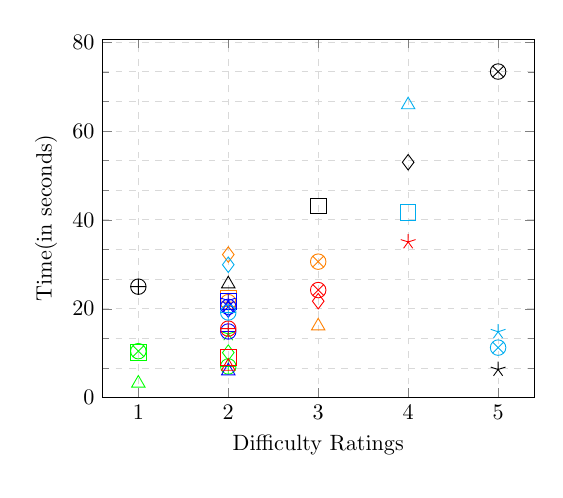
\begin{tikzpicture}[scale=0.80]
	\begin{axis}[%
	xlabel={Difficulty Ratings},
    ylabel={Time(in seconds)},
    ymin=0,
    minor y tick num=2,
    grid style={dashed,gray!30},
    ymajorgrids=true,
    xmajorgrids=true,
    yminorgrids=true,
    only marks,
    scatter,
    mark size=3.5pt,
    scatter src=explicit symbolic,
	scatter/classes={
		a={mark=square,draw=gray},
		b={mark=triangle,draw=gray},
		c={mark=otimes,draw=gray},
		x={mark=diamond,draw=gray},
	    y={mark=oplus,draw=gray},
		z={mark=star,draw=gray},
		q1sRa={mark=square,draw=green},
	    q1sT={mark=triangle,draw=green},
		q1sRo={mark=otimes,draw=green},
		q1cRa={mark=diamond,draw=green},
	    q1cT={mark=oplus,draw=green},
		q1cRo={mark=star,draw=green},
		q2sRa={mark=square,draw=orange},
	    q2sT={mark=triangle,draw=orange},
		q2sRo={mark=otimes,draw=orange},
		q2cRa={mark=diamond,draw=orange},
	    q2cT={mark=oplus,draw=orange},
		q2cRo={mark=star,draw=orange},
		q3sRa={mark=square,draw=blue},
	    q3sT={mark=triangle,draw=blue},
		q3sRo={mark=otimes,draw=blue},
		q3cRa={mark=diamond,draw=blue},
	    q3cT={mark=oplus,draw=blue},
		q3cRo={mark=star,draw=blue},
		q4sRa={mark=square,draw=red},
	    q4sT={mark=triangle,draw=red},
		q4sRo={mark=otimes,draw=red},
		q4cRa={mark=diamond,draw=red},
	    q4cT={mark=oplus,draw=red},
		q4cRo={mark=star,draw=red},
		q5sRa={mark=square,draw=black},
	    q5sT={mark=triangle,draw=black},
		q5sRo={mark=otimes,draw=black},
		q5cRa={mark=diamond,draw=black},
	    q5cT={mark=oplus,draw=black},
		q5cRo={mark=star,draw=black},
		q6sRa={mark=square,draw=cyan},
	    q6sT={mark=triangle,draw=cyan},
		q6sRo={mark=otimes,draw=cyan},
		q6cRa={mark=diamond,draw=cyan},
	    q6cT={mark=oplus,draw=cyan},
		q6cRo={mark=star,draw=cyan}}]
	\addplot[scatter,only marks,%
		scatter src=explicit symbolic]%
	table[meta=label] {
x         y         label
		
		
1	10.2	q1sRa
1	3.23	q1sT
1	10.45	q1sRo
		
2	10.12	q1cRa
2	7.02	q1cT
2	14.33	q1cRo
		
		
2	22.27	q2sRa
3	16.11	q2sT
3	30.6	q2sRo
		
2	32.19	q2cRa
2	21.49	q2cT
		
		
2	21.64	q3sRa
2	6	q3sT
2	20.43	q3sRo
		
2	19.82	q3cRa
2	14.88	q3cT
2	21.84	q3cRo
		
		
2	9.07	q4sRa
2	7.04	q4sT
3	24.2	q4sRo
		
3	21.71	q4cRa
2	15.53	q4cT
4	35.03	q4cRo
		
		
3	43.14	q5sRa
2	25.58	q5sT
5	73.39	q5sRo
		
4	52.97	q5cRa
1	24.97	q5cT
5	6.33	q5cRo
		
		
4	41.64	q6sRa
4	65.88	q6sT
5	11.25	q6sRo
		
2	29.91	q6cRa
2	19.16	q6cT
5	14.82	q6cRo

};
\end{axis}
	
\begin{axis}[
    xmin=0,
    xmax=100,
    ymin=1,
    ymax=6,
    hide axis,
    only marks,
    ]
\foreach \i in {0,...,6} {
        \addplot+ [mark=*] coordinates { (0,0) };
     }
    \end{axis}
\end{tikzpicture}
\caption{Difficulty rating and time measurements for interviewee 2} 
\label{figure:interviewee2}
\vspace{\baselineskip}
\end{minipage}



\end{adjustbox}
\end{figure}

\begin{figure}[H]
\centering
\begin{adjustbox}{width=1\textwidth}
\begin{minipage}[8cm]{.44\textwidth}
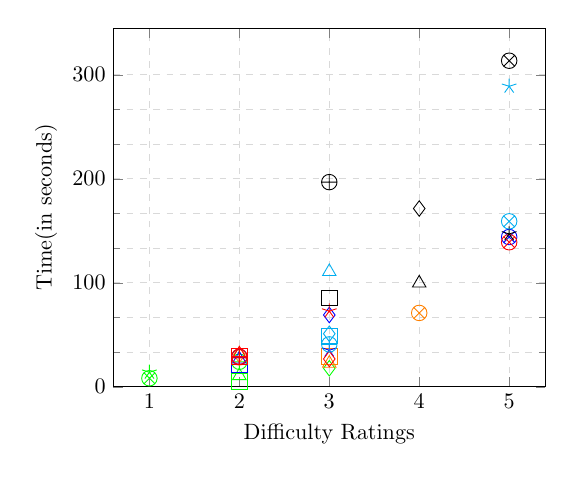
\begin{tikzpicture}[scale=0.80]
	\begin{axis}[%
	xlabel={Difficulty Ratings},
    ylabel={Time(in seconds)},
    ymin=0,
    minor y tick num=2,
    grid style={dashed,gray!30},
    ymajorgrids=true,
    xmajorgrids=true,
    yminorgrids=true,
    only marks,
    scatter,
    mark size=3.5pt,
    scatter src=explicit symbolic,
	scatter/classes={
		a={mark=square,draw=gray},
		b={mark=triangle,draw=gray},
		c={mark=otimes,draw=gray},
		x={mark=diamond,draw=gray},
	    y={mark=oplus,draw=gray},
		z={mark=star,draw=gray},
		q1sRa={mark=square,draw=green},
	    q1sT={mark=triangle,draw=green},
		q1sRo={mark=otimes,draw=green},
		q1cRa={mark=diamond,draw=green},
	    q1cT={mark=oplus,draw=green},
		q1cRo={mark=star,draw=green},
		q2sRa={mark=square,draw=orange},
	    q2sT={mark=triangle,draw=orange},
		q2sRo={mark=otimes,draw=orange},
		q2cRa={mark=diamond,draw=orange},
	    q2cT={mark=oplus,draw=orange},
		q2cRo={mark=star,draw=orange},
		q3sRa={mark=square,draw=blue},
	    q3sT={mark=triangle,draw=blue},
		q3sRo={mark=otimes,draw=blue},
		q3cRa={mark=diamond,draw=blue},
	    q3cT={mark=oplus,draw=blue},
		q3cRo={mark=star,draw=blue},
		q4sRa={mark=square,draw=red},
	    q4sT={mark=triangle,draw=red},
		q4sRo={mark=otimes,draw=red},
		q4cRa={mark=diamond,draw=red},
	    q4cT={mark=oplus,draw=red},
		q4cRo={mark=star,draw=red},
		q5sRa={mark=square,draw=black},
	    q5sT={mark=triangle,draw=black},
		q5sRo={mark=otimes,draw=black},
		q5cRa={mark=diamond,draw=black},
	    q5cT={mark=oplus,draw=black},
		q5cRo={mark=star,draw=black},
		q6sRa={mark=square,draw=cyan},
	    q6sT={mark=triangle,draw=cyan},
		q6sRo={mark=otimes,draw=cyan},
		q6cRa={mark=diamond,draw=cyan},
	    q6cT={mark=oplus,draw=cyan},
		q6cRo={mark=star,draw=cyan}},]
	\addplot[scatter,only marks,%
		scatter src=explicit symbolic]%
	table[meta=label] {
x         y         label
2	5.024	q1sRa
2	10.598	q1sT
1	8.192	q1sRo
		
3	17.776	q1cRa
2	24.036	q1cT
1	13.924	q1cRo
		
		
3	28.976	q2sRa
3	22.55	q2sT
4	71.008	q2sRo
		
2	30.775	q2cRa
2	28.218	q2cT
		
		
2	21.04	q3sRa
2	26.556	q3sT
5	144.0	q3sRo
		
3	69.0	q3cRa
2	28.73	q3cT
3	35.122	q3cRo
		
		
2	28.97	q4sRa
2	31.51	q4sT
5	139.0	q4sRo
		
3	26.741	q4cRa
2	28.969	q4cT
3	72.741	q4cRo
		
		
3	85.5	q5sRa
4	99.7	q5sT
5	313.555	q5sRo
		
4	171.4	q5cRa
3	196.8	q5cT
5	146.903	q5cRo
		
		
3	49.043	q6sRa
3	110.686	q6sT
5	159.1	q6sRo
		
3	51.01	q6cRa
3	40.757	q6cT
5	288.940	q6cRo
};
\end{axis}
	
\begin{axis}[
    xmin=0,
    xmax=100,
    ymin=1,
    ymax=6,
    hide axis,
    only marks,
    ]
\foreach \i in {0,...,6} {
        \addplot+ [mark=*] coordinates { (0,0) };
     }
    \end{axis}
\end{tikzpicture}
\caption{Difficulty rating and time measurements for interviewee 3}\label{figure:interviewee3}
\vspace{\baselineskip}
\end{minipage}
\begin{minipage}[8cm]{.44\textwidth}
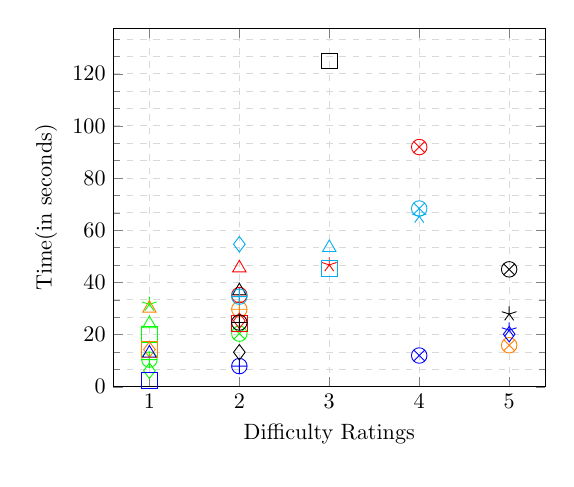
\begin{tikzpicture}[scale=0.80]
	\begin{axis}[%
	xlabel={Difficulty Ratings},
    ylabel={Time(in seconds)},
    ymin=0,
    minor y tick num=2,
    grid style={dashed,gray!30},
    ymajorgrids=true,
    xmajorgrids=true,
    yminorgrids=true,
    only marks,
    scatter,
    mark size=3.5pt,
    scatter src=explicit symbolic,
	scatter/classes={
		a={mark=square,draw=gray},
		b={mark=triangle,draw=gray},
		c={mark=otimes,draw=gray},
		x={mark=diamond,draw=gray},
	    y={mark=oplus,draw=gray},
		z={mark=star,draw=gray},
		q1sRa={mark=square,draw=green},
	    q1sT={mark=triangle,draw=green},
		q1sRo={mark=otimes,draw=green},
		q1cRa={mark=diamond,draw=green},
	    q1cT={mark=oplus,draw=green},
		q1cRo={mark=star,draw=green},
		q2sRa={mark=square,draw=orange},
	    q2sT={mark=triangle,draw=orange},
		q2sRo={mark=otimes,draw=orange},
		q2cRa={mark=diamond,draw=orange},
	    q2cT={mark=oplus,draw=orange},
		q2cRo={mark=star,draw=orange},
		q3sRa={mark=square,draw=blue},
	    q3sT={mark=triangle,draw=blue},
		q3sRo={mark=otimes,draw=blue},
		q3cRa={mark=diamond,draw=blue},
	    q3cT={mark=oplus,draw=blue},
		q3cRo={mark=star,draw=blue},
		q4sRa={mark=square,draw=red},
	    q4sT={mark=triangle,draw=red},
		q4sRo={mark=otimes,draw=red},
		q4cRa={mark=diamond,draw=red},
	    q4cT={mark=oplus,draw=red},
		q4cRo={mark=star,draw=red},
		q5sRa={mark=square,draw=black},
	    q5sT={mark=triangle,draw=black},
		q5sRo={mark=otimes,draw=black},
		q5cRa={mark=diamond,draw=black},
	    q5cT={mark=oplus,draw=black},
		q5cRo={mark=star,draw=black},
		q6sRa={mark=square,draw=cyan},
	    q6sT={mark=triangle,draw=cyan},
		q6sRo={mark=otimes,draw=cyan},
		q6cRa={mark=diamond,draw=cyan},
	    q6cT={mark=oplus,draw=cyan},
		q6cRo={mark=star,draw=cyan}},]
	\addplot[scatter,only marks,%
		scatter src=explicit symbolic]%
	table[meta=label] {
x         y         label
		
		
1	20.089	q1sRa
1	24.125	q1sT
2	20.362	q1sRo
		
1	6.124	q1cRa
1	10.416	q1cT
1	31.608	q1cRo
		
		
1	14.328	q2sRa
1	30.085	q2sT
5	15.913	q2sRo
		
1	14.296	q2cRa
2	29.725	q2cT
		
		
1	2.357	q3sRa
1	12.884	q3sT
4	11.979	q3sRo
		
5	20.154	q3cRa
2	7.927	q3cT
5	21.694	q3cRo
		
		
2	24.296	q4sRa
2	45.527	q4sT
4	91.9	q4sRo
		
2	25.298	q4cRa
2	35.165	q4cT
3	46.726	q4cRo
		
		
3	125.0	q5sRa
2	36.758	q5sT
5	45.017	q5sRo
		
2	13.229	q5cRa
2	24.62	q5cT
5	27.879	q5cRo
		
		
3	45.44	q6sRa
3	53.34	q6sT
4	68.346	q6sRo
		
2	54.65	q6cRa
2	34.56	q6cT
4	65.34	q6cRo

};
\end{axis}
	
\begin{axis}[
    xmin=0,
    xmax=100,
    ymin=1,
    ymax=6,
    hide axis,
    only marks,]
\foreach \i in {0,...,6} {
        \addplot+ [mark=*] coordinates { (0,0) };
     }
    \end{axis}
\end{tikzpicture}
\caption{Difficulty rating and time measurements for interviewee 4}\label{figure:interviewee4}
\vspace{\baselineskip}
\end{minipage}
\end{adjustbox}
\end{figure}

\begin{figure}[H]
\centering
\begin{adjustbox}{width=1\textwidth}
\begin{minipage}[8cm]{.44\textwidth}
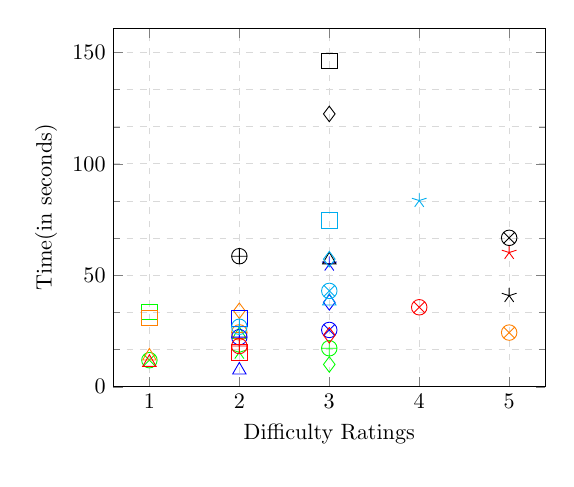
\begin{tikzpicture}[scale=0.80]
	\begin{axis}[%
	xlabel={Difficulty Ratings},
    ylabel={Time(in seconds)},
    ymin=0,
    minor y tick num=2,
    grid style={dashed,gray!30},
    ymajorgrids=true,
    xmajorgrids=true,
    yminorgrids=true,
    only marks,
    scatter,
    mark size=3.5pt,
    scatter src=explicit symbolic,
	scatter/classes={
		a={mark=square,draw=gray},
		b={mark=triangle,draw=gray},
		c={mark=otimes,draw=gray},
		x={mark=diamond,draw=gray},
	    y={mark=oplus,draw=gray},
		z={mark=star,draw=gray},
		q1sRa={mark=square,draw=green},
	    q1sT={mark=triangle,draw=green},
		q1sRo={mark=otimes,draw=green},
		q1cRa={mark=diamond,draw=green},
	    q1cT={mark=oplus,draw=green},
		q1cRo={mark=star,draw=green},
		q2sRa={mark=square,draw=orange},
	    q2sT={mark=triangle,draw=orange},
		q2sRo={mark=otimes,draw=orange},
		q2cRa={mark=diamond,draw=orange},
	    q2cT={mark=oplus,draw=orange},
		q2cRo={mark=star,draw=orange},
		q3sRa={mark=square,draw=blue},
	    q3sT={mark=triangle,draw=blue},
		q3sRo={mark=otimes,draw=blue},
		q3cRa={mark=diamond,draw=blue},
	    q3cT={mark=oplus,draw=blue},
		q3cRo={mark=star,draw=blue},
		q4sRa={mark=square,draw=red},
	    q4sT={mark=triangle,draw=red},
		q4sRo={mark=otimes,draw=red},
		q4cRa={mark=diamond,draw=red},
	    q4cT={mark=oplus,draw=red},
		q4cRo={mark=star,draw=red},
		q5sRa={mark=square,draw=black},
	    q5sT={mark=triangle,draw=black},
		q5sRo={mark=otimes,draw=black},
		q5cRa={mark=diamond,draw=black},
	    q5cT={mark=oplus,draw=black},
		q5cRo={mark=star,draw=black},
		q6sRa={mark=square,draw=cyan},
	    q6sT={mark=triangle,draw=cyan},
		q6sRo={mark=otimes,draw=cyan},
		q6cRa={mark=diamond,draw=cyan},
	    q6cT={mark=oplus,draw=cyan},
		q6cRo={mark=star,draw=cyan}},]
	\addplot[scatter,only marks,%
		scatter src=explicit symbolic]%
	table[meta=label] {
x         y         label
1	33.57	q1sRa
2	23.46	q1sT
1	11.93	q1sRo
		
3	10.01	q1cRa
3	17.28	q1cT
2	15.46	q1cRo
		
		
1	30.98	q2sRa
1	13.76	q2sT
5	24.32	q2sRo
		
2	34.1	q2cRa
2	24.4	q2cT
		
		
2	30.68	q3sRa
2	7.45	q3sT
3	25.5	q3sRo
		
3	37.88	q3cRa
2	22.25	q3cT
3	54.98	q3cRo
		
		
2	15.45	q4sRa
1	10.9	q4sT
4	35.67	q4sRo
		
3	23.11	q4cRa
2	18.29	q4cT
5	60.23	q4cRo
		
		
3	146.31	q5sRa
3	56.9	q5sT
5	66.84	q5sRo
		
3	122.44	q5cRa
2	58.59	q5cT
5	40.88	q5cRo
		
		
3	74.57	q6sRa
3	38.44	q6sT
3	43.02	q6sRo
		
3	57.25	q6cRa
2	26.93	q6cT
4	83.55	q6cRo


};
\end{axis}
	
\begin{axis}[
    xmin=0,
    xmax=100,
    ymin=1,
    ymax=6,
    hide axis,
    only marks,
    ]
\foreach \i in {0,...,6} {
        \addplot+ [mark=*] coordinates { (0,0) };
     }
    \end{axis}
\end{tikzpicture}
\caption{Difficulty rating and time measurements for interviewee 5}\label{figure:interviewee5}
\vspace{\baselineskip}
\end{minipage}
\begin{minipage}[8cm]{.44\textwidth}
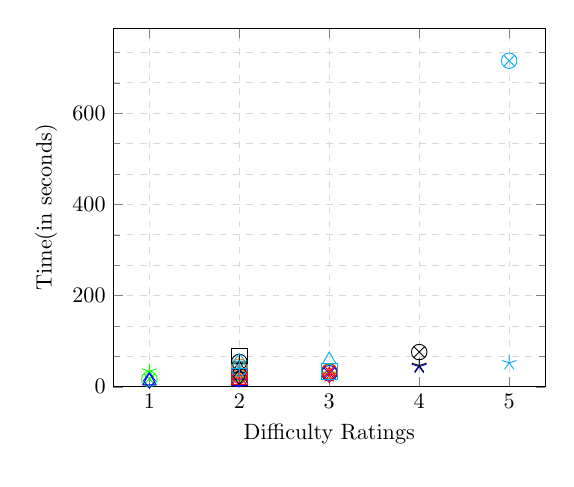
\begin{tikzpicture}[scale=0.80]
	\begin{axis}[%
	xlabel={Difficulty Ratings},
    ylabel={Time(in seconds)},
    ymin=0,
    minor y tick num=2,
    grid style={dashed,gray!30},
    ymajorgrids=true,
    xmajorgrids=true,
    yminorgrids=true,
    only marks,
    scatter,
    mark size=3.5pt,
    scatter src=explicit symbolic,
	scatter/classes={
		a={mark=square,draw=gray},
		b={mark=triangle,draw=gray},
		c={mark=otimes,draw=gray},
		x={mark=diamond,draw=gray},
	    y={mark=oplus,draw=gray},
		z={mark=star,draw=gray},
		q1sRa={mark=square,draw=green},
	    q1sT={mark=triangle,draw=green},
		q1sRo={mark=otimes,draw=green},
		q1cRa={mark=diamond,draw=green},
	    q1cT={mark=oplus,draw=green},
		q1cRo={mark=star,draw=green},
		q2sRa={mark=square,draw=orange},
	    q2sT={mark=triangle,draw=orange},
		q2sRo={mark=otimes,draw=orange},
		q2cRa={mark=diamond,draw=orange},
	    q2cT={mark=oplus,draw=orange},
		q2cRo={mark=star,draw=orange},
		q3sRa={mark=square,draw=blue},
	    q3sT={mark=triangle,draw=blue},
		q3sRo={mark=otimes,draw=blue},
		q3cRa={mark=diamond,draw=blue},
	    q3cT={mark=oplus,draw=blue},
		q3cRo={mark=star,draw=blue},
		q4sRa={mark=square,draw=red},
	    q4sT={mark=triangle,draw=red},
		q4sRo={mark=otimes,draw=red},
		q4cRa={mark=diamond,draw=red},
	    q4cT={mark=oplus,draw=red},
		q4cRo={mark=star,draw=red},
		q5sRa={mark=square,draw=black},
	    q5sT={mark=triangle,draw=black},
		q5sRo={mark=otimes,draw=black},
		q5cRa={mark=diamond,draw=black},
	    q5cT={mark=oplus,draw=black},
		q5cRo={mark=star,draw=black},
		q6sRa={mark=square,draw=cyan},
	    q6sT={mark=triangle,draw=cyan},
		q6sRo={mark=otimes,draw=cyan},
		q6cRa={mark=diamond,draw=cyan},
	    q6cT={mark=oplus,draw=cyan},
		q6cRo={mark=star,draw=cyan}}]
	\addplot[scatter,only marks,%
		scatter src=explicit symbolic]%
	table[meta=label] {
x         y         label
2	36.969	q1sRa
2	22.17	q1sT
1	16.967	q1sRo
		
2	24.232	q1cRa
3	32.167	q1cT
1	33.992	q1cRo
		
		
2	34.977	q2sRa
2	25.743	q2sT
2	43.967	q2sRo
		
2	18.869	q2cRa
2	36.871	q2cT
		
		
2	20.768	q3sRa
1	12.771	q3sT
3	29.559	q3sRo
		
1	13.532	q3cRa
2	16.686	q3cT
4	44.234	q3cRo
		
		
2	22.515	q4sRa
2	13.725	q4sT
3	33.804	q4sRo
		
3	25.71	q4cRa
2	24.5	q4cT
3	25.446	q4cRo
		
		
2	 67.798	q5sRa
2	40.329	q5sT
4	 76.052	q5sRo
		
2	21.658	q5cRa
2	54.374	q5cT
4	46.601	q5cRo
		
3	33.894	q6sRa
3	59.25	q6sT
5	715.016	q6sRo
		
2	55.654	q6cRa
2	39.917	q6cT
5	52.343	q6cRo
};
\end{axis}
	
\begin{axis}[
    xmin=0,
    xmax=100,
    ymin=1,
    ymax=6,
    hide axis,
    only marks,
    ]
\foreach \i in {0,...,6} {
        \addplot+ [mark=*] coordinates { (0,0) };
     }
    \end{axis}
\end{tikzpicture}
\caption{Difficulty rating and time measurements for interviewee 6}\label{figure:interviewee6}
\vspace{\baselineskip}
\end{minipage}
\end{adjustbox}
\end{figure}

\begin{figure}[H]
\centering
\begin{adjustbox}{width=1\textwidth}
\begin{minipage}[8cm]{.44\textwidth}
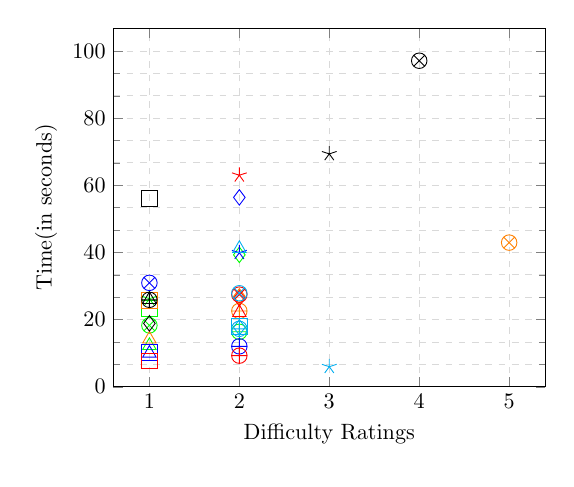
\begin{tikzpicture}[scale=0.80]
	\begin{axis}[%
	xlabel={Difficulty Ratings},
    ylabel={Time(in seconds)},
    ymin=0,
    minor y tick num=2,
    grid style={dashed,gray!30},
    ymajorgrids=true,
    xmajorgrids=true,
    yminorgrids=true,
    only marks,
    scatter,
    mark size=3.5pt,
    scatter src=explicit symbolic,
	scatter/classes={
		a={mark=square,draw=gray},
		b={mark=triangle,draw=gray},
		c={mark=otimes,draw=gray},
		x={mark=diamond,draw=gray},
	    y={mark=oplus,draw=gray},
		z={mark=star,draw=gray},
		q1sRa={mark=square,draw=green},
	    q1sT={mark=triangle,draw=green},
		q1sRo={mark=otimes,draw=green},
		q1cRa={mark=diamond,draw=green},
	    q1cT={mark=oplus,draw=green},
		q1cRo={mark=star,draw=green},
		q2sRa={mark=square,draw=orange},
	    q2sT={mark=triangle,draw=orange},
		q2sRo={mark=otimes,draw=orange},
		q2cRa={mark=diamond,draw=orange},
	    q2cT={mark=oplus,draw=orange},
		q2cRo={mark=star,draw=orange},
		q3sRa={mark=square,draw=blue},
	    q3sT={mark=triangle,draw=blue},
		q3sRo={mark=otimes,draw=blue},
		q3cRa={mark=diamond,draw=blue},
	    q3cT={mark=oplus,draw=blue},
		q3cRo={mark=star,draw=blue},
		q4sRa={mark=square,draw=red},
	    q4sT={mark=triangle,draw=red},
		q4sRo={mark=otimes,draw=red},
		q4cRa={mark=diamond,draw=red},
	    q4cT={mark=oplus,draw=red},
		q4cRo={mark=star,draw=red},
		q5sRa={mark=square,draw=black},
	    q5sT={mark=triangle,draw=black},
		q5sRo={mark=otimes,draw=black},
		q5cRa={mark=diamond,draw=black},
	    q5cT={mark=oplus,draw=black},
		q5cRo={mark=star,draw=black},
		q6sRa={mark=square,draw=cyan},
	    q6sT={mark=triangle,draw=cyan},
		q6sRo={mark=otimes,draw=cyan},
		q6cRa={mark=diamond,draw=cyan},
	    q6cT={mark=oplus,draw=cyan},
		q6cRo={mark=star,draw=cyan}},]
	\addplot[scatter,only marks,%
		scatter src=explicit symbolic]%
	table[meta=label] {
x         y         label
1	23.266	q1sRa
1	12.262	q1sT
1	18.282	q1sRo
		
2	39.292	q1cRa
2	16.376	q1cT
1	26.229	q1cRo
		
		
1	25.712	q2sRa
1	14.18	q2sT
5	42.934	q2sRo
		
2	26.911	q2cRa
2	22.574	q2cT
		
		
1	10.217	q3sRa
1	9.968	q3sT
1	30.947	q3sRo
		
2	56.401	q3cRa
2	12.044	q3cT
2	39.93	q3cRo
		
		
1	7.731	q4sRa
2	22.087	q4sT
2	27.443	q4sRo
		
2	26.379	q4cRa
2	9.274	q4cT
2	63.0	q4cRo
		
		
1	56.019	q5sRa
1	25.968	q5sT
4	97.1	q5sRo
		
1	18.88	q5cRa
1	25.893	q5cT
3	69.359	q5cRo
		
		
2	17.963	q6sRa
2	41.166	q6sT
2	27.851	q6sRo
		
2	17.708	q6cRa
2	17.255	q6cT
3	5.981	q6cRo

};
\end{axis}
	
\begin{axis}[
    xmin=0,
    xmax=100,
    ymin=1,
    ymax=6,
    hide axis,
    only marks,
    ]
\foreach \i in {0,...,6} {
        \addplot+ [mark=*] coordinates { (0,0) };
     }
    \end{axis}
\end{tikzpicture}
\caption{Difficulty rating and time measurements for interviewee 7}\label{figure:interviewee7}
\vspace{\baselineskip}
\end{minipage}
\begin{minipage}[8cm]{.44\textwidth}
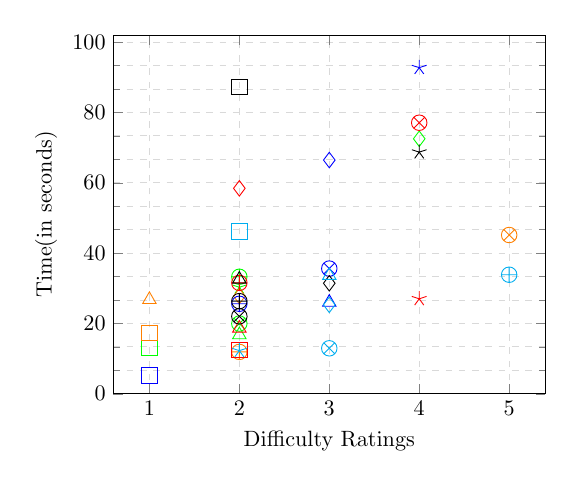
\begin{tikzpicture}[scale=0.80]
	\begin{axis}[%
	xlabel={Difficulty Ratings},
    ylabel={Time(in seconds)},
    ymin=0,
    minor y tick num=2,
    grid style={dashed,gray!30},
    ymajorgrids=true,
    xmajorgrids=true,
    yminorgrids=true,
    only marks,
    scatter,
    mark size=3.5pt,
    scatter src=explicit symbolic,
	scatter/classes={
		a={mark=square,draw=gray},
		b={mark=triangle,draw=gray},
		c={mark=otimes,draw=gray},
		x={mark=diamond,draw=gray},
	    y={mark=oplus,draw=gray},
		z={mark=star,draw=gray},
		q1sRa={mark=square,draw=green},
	    q1sT={mark=triangle,draw=green},
		q1sRo={mark=otimes,draw=green},
		q1cRa={mark=diamond,draw=green},
	    q1cT={mark=oplus,draw=green},
		q1cRo={mark=star,draw=green},
		q2sRa={mark=square,draw=orange},
	    q2sT={mark=triangle,draw=orange},
		q2sRo={mark=otimes,draw=orange},
		q2cRa={mark=diamond,draw=orange},
	    q2cT={mark=oplus,draw=orange},
		q2cRo={mark=star,draw=orange},
		q3sRa={mark=square,draw=blue},
	    q3sT={mark=triangle,draw=blue},
		q3sRo={mark=otimes,draw=blue},
		q3cRa={mark=diamond,draw=blue},
	    q3cT={mark=oplus,draw=blue},
		q3cRo={mark=star,draw=blue},
		q4sRa={mark=square,draw=red},
	    q4sT={mark=triangle,draw=red},
		q4sRo={mark=otimes,draw=red},
		q4cRa={mark=diamond,draw=red},
	    q4cT={mark=oplus,draw=red},
		q4cRo={mark=star,draw=red},
		q5sRa={mark=square,draw=black},
	    q5sT={mark=triangle,draw=black},
		q5sRo={mark=otimes,draw=black},
		q5cRa={mark=diamond,draw=black},
	    q5cT={mark=oplus,draw=black},
		q5cRo={mark=star,draw=black},
		q6sRa={mark=square,draw=cyan},
	    q6sT={mark=triangle,draw=cyan},
		q6sRo={mark=otimes,draw=cyan},
		q6cRa={mark=diamond,draw=cyan},
	    q6cT={mark=oplus,draw=cyan},
		q6cRo={mark=star,draw=cyan}},]
	\addplot[scatter,only marks,%
		scatter src=explicit symbolic]%
	table[meta=label] {
x         y         label
1	12.97	q1sRa
2	16.75	q1sT
2	19.96	q1sRo
		
4	72.52	q1cRa
2	33.27	q1cT
2	30.29	q1cRo
		
		
1	17.26	q2sRa
1	26.77	q2sT
5	45.15	q2sRo
		
2	27.76	q2cRa
2	11.9	q2cT
		
		
1	5.23	q3sRa
3	26	    q3sT
3	35.6	q3sRo
		
3	66.47	q3cRa
2	25.58	q3cT
4	92.75	q3cRo
		
		
2	12.42	q4sRa
2	18.63	q4sT
4	77.09	q4sRo
		
2	58.42	q4cRa
2	31.53	q4cT
4	27	    q4cRo
		
		
2	87.21	q5sRa
2	32.57	q5sT
2	22.02	q5sRo
		
3	31.42	q5cRa
2	26.34	q5cT
4	68.73	q5cRo
		
		
2	46.1	q6sRa
3	33.62	q6sT
3	12.92	q6sRo
		
3	25.29	q6cRa
5	33.85	q6cT
2	12.25	q6cRo
};
\end{axis}
	
\begin{axis}[
    xmin=0,
    xmax=100,
    ymin=1,
    ymax=6,
    hide axis,
    only marks,
    ]
\foreach \i in {0,...,6} {
        \addplot+ [mark=*] coordinates { (0,0) };
     }
    \end{axis}
\end{tikzpicture}
\caption{Difficulty rating and time measurements for interviewee 8}\label{figure:interviewee8}
\vspace{\baselineskip}
\end{minipage}
\end{adjustbox}
\end{figure}

\begin{figure}[ht]
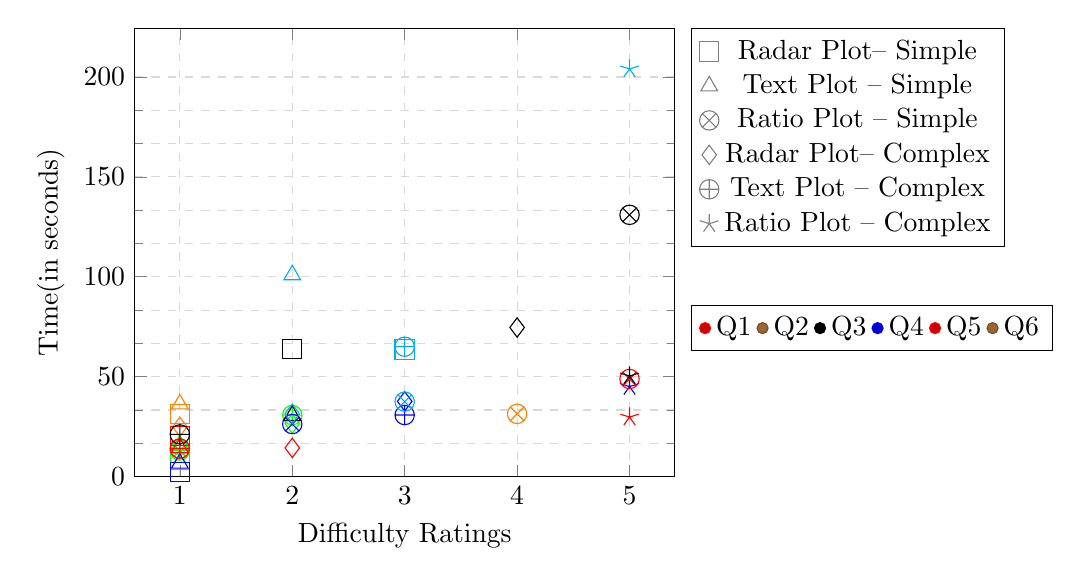
\begin{tikzpicture}
	\begin{axis}[%
	xlabel={Difficulty Ratings},
    ylabel={Time(in seconds)},
    ymin=0,
    minor y tick num=2,
    grid style={dashed,gray!30},
    ymajorgrids=true,
    xmajorgrids=true,
    yminorgrids=true,
    only marks,
    scatter,
    mark size=3.5pt,
    scatter src=explicit symbolic,
	scatter/classes={
		a={mark=square,draw=gray},
		b={mark=triangle,draw=gray},
		c={mark=otimes,draw=gray},
		x={mark=diamond,draw=gray},
	    y={mark=oplus,draw=gray},
		z={mark=star,draw=gray},
		q1sRa={mark=square,draw=green},
	    q1sT={mark=triangle,draw=green},
		q1sRo={mark=otimes,draw=green},
		q1cRa={mark=diamond,draw=green},
	    q1cT={mark=oplus,draw=green},
		q1cRo={mark=star,draw=green},
		q2sRa={mark=square,draw=orange},
	    q2sT={mark=triangle,draw=orange},
		q2sRo={mark=otimes,draw=orange},
		q2cRa={mark=diamond,draw=orange},
	    q2cT={mark=oplus,draw=orange},
		q2cRo={mark=star,draw=orange},
		q3sRa={mark=square,draw=blue},
	    q3sT={mark=triangle,draw=blue},
		q3sRo={mark=otimes,draw=blue},
		q3cRa={mark=diamond,draw=blue},
	    q3cT={mark=oplus,draw=blue},
		q3cRo={mark=star,draw=blue},
		q4sRa={mark=square,draw=red},
	    q4sT={mark=triangle,draw=red},
		q4sRo={mark=otimes,draw=red},
		q4cRa={mark=diamond,draw=red},
	    q4cT={mark=oplus,draw=red},
		q4cRo={mark=star,draw=red},
		q5sRa={mark=square,draw=black},
	    q5sT={mark=triangle,draw=black},
		q5sRo={mark=otimes,draw=black},
		q5cRa={mark=diamond,draw=black},
	    q5cT={mark=oplus,draw=black},
		q5cRo={mark=star,draw=black},
		q6sRa={mark=square,draw=cyan},
	    q6sT={mark=triangle,draw=cyan},
		q6sRo={mark=otimes,draw=cyan},
		q6cRa={mark=diamond,draw=cyan},
	    q6cT={mark=oplus,draw=cyan},
		q6cRo={mark=star,draw=cyan}},
	     legend entries={
            Radar Plot-- Simple,
            Text Plot -- Simple,
            Ratio Plot -- Simple,
            Radar Plot-- Complex,
            Text Plot -- Complex,
            Ratio Plot -- Complex%
        },
        legend pos=outer north east,]
	\addplot[scatter,only marks,%
		scatter src=explicit symbolic]%
	table[meta=label] {
x         y         label
1	8.19	q1sRa
1	15.81	q1sT
1	13.01	q1sRo
		
2	26.52	q1cRa
2	30.77	q1cT
1	10.91	q1cRo
		
		
1	31.33	q2sRa
1	36.28	q2sT
4	31.37	q2sRo
		
1	24.92	q2cRa
1	13.77	q2cT
		
		
1	2.32	q3sRa
1	6.62	q3sT
2	26.28	q3sRo
		
3	37.64	q3cRa
3	30.79	q3cT
5	45.01	q3cRo
		
		
1	20.42	q4sRa
1	14.46	q4sT
5	48.84	q4sRo
		
2	14.34	q4cRa
1	14.04	q4cT
5	29.74	q4cRo
		
		
2	63.85	q5sRa
2	30.57	q5sT
5	131.0	q5sRo
		
4	74.6	q5cRa
1	21.09	q5cT
5	50.3	q5cRo
		
		
3	63.56	q6sRa
2	100.91	q6sT
3	37.49	q6sRo
		
2	31.43	q6cRa
3	65.0	q6cT
5	204.0	q6cRo

};
\end{axis}
	
\begin{axis}[
    xmin=0,
    xmax=100,
    ymin=1,
    ymax=6,
    hide axis,
    only marks,
    legend entries={
     ,   % the dummy plot should not show up in the legend
     Q1,Q2,Q3,Q4,Q5,Q6%
    },
    legend pos=outer north east,
    legend style={
            legend columns=-1, yshift=-100pt,
        },
    ]
\foreach \i in {0,...,6} {
        \addplot+ [mark=*] coordinates { (0,0) };
     }
    \end{axis}
\end{tikzpicture}
\label{figure:interviewee9}
\caption[Difficulty rating and time measurements for interviewee 9]{Difficulty rating and time measurements for interviewee 9} 
\end{figure}


\section{Questionnaire}
\label{appendix:questionnaire}
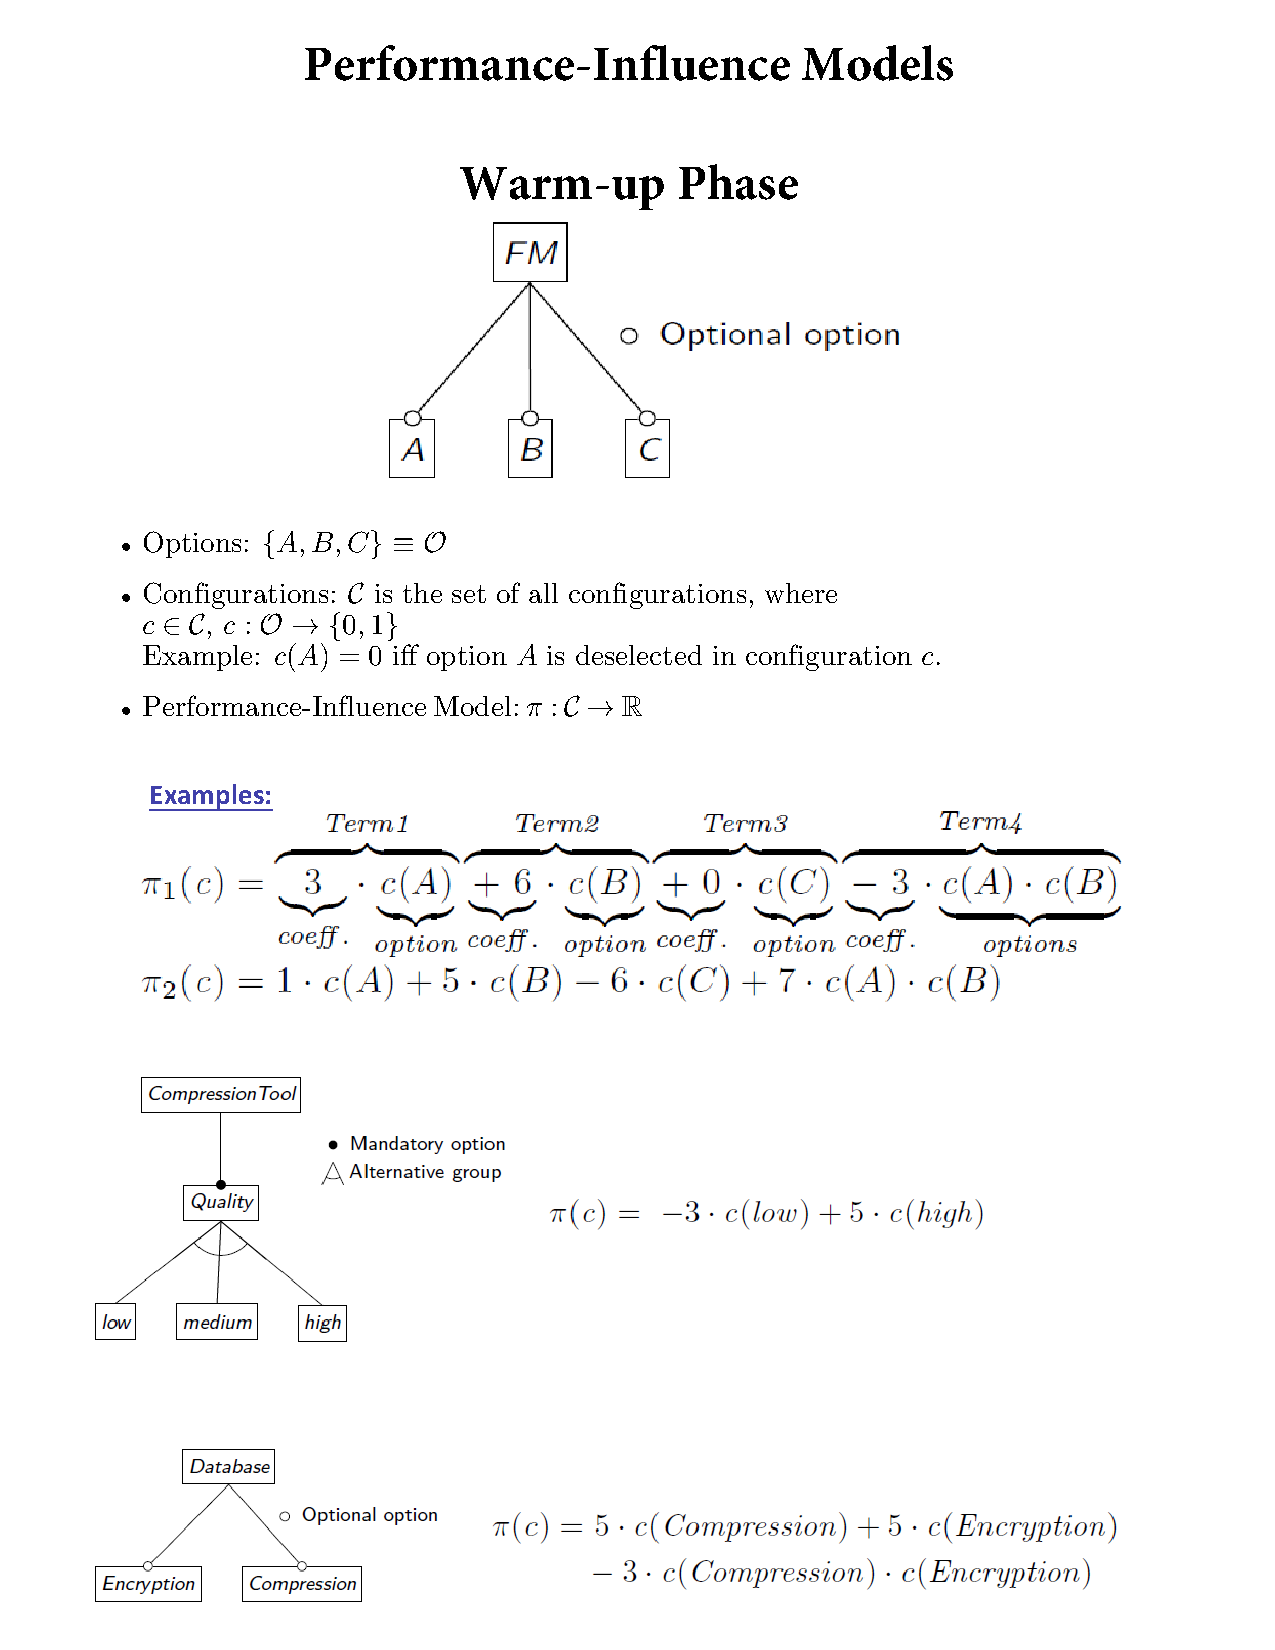
\includepdf[pages=-]{literature/Interview_Questionnaire.pdf}
